\section*{Installing Unity}
To run or build the provided source code two things need to be installed on the system:

\begin{enumerate}
    \item Unity - the editor in which the provided code can be opened. To install follow the instructions at \url{https://docs.unity3d.com/Manual/InstallingUnity.html} % Need to check if it will work with any version
    \item Steam \acrshort{vr} - a library that provides \acrshort{vr} support for the project. To install it, Steam must be installed first before Steam \acrshort{vr} can be installed: \url{http://store.steampowered.com/steamvr}
\end{enumerate}

After the above components are installed on the system, the provided source code can be opened in the Unity editor. After opening it in the Unity editor, the furniture assets need to be prepared in order for the Object Tool to work as intended. To do this click Assets > Build AssetBundles from the menu bar. Only then the project can be run on the local computer.

\section*{Installing the project}
To build the project with Unity select File > Build Settings... This will open a new window in which you can specify some build details. Click Build to build the project as a standalone piece of software in the specified location. To supply the build project with default furniture assets, copy \verb|AssetBundles\sample| file from the source code and copy it into \verb|main_Data\AssetBundles| directory in the build location. The program can then be execute by running the newly created executable main file.

\section*{Using the program}
The following section will describe different parts of using the application. The image will figure~\ref{fig:vive_controllers} will be used as a reference to explain what button to press when using the program.

\begin{figure}[!ht]
 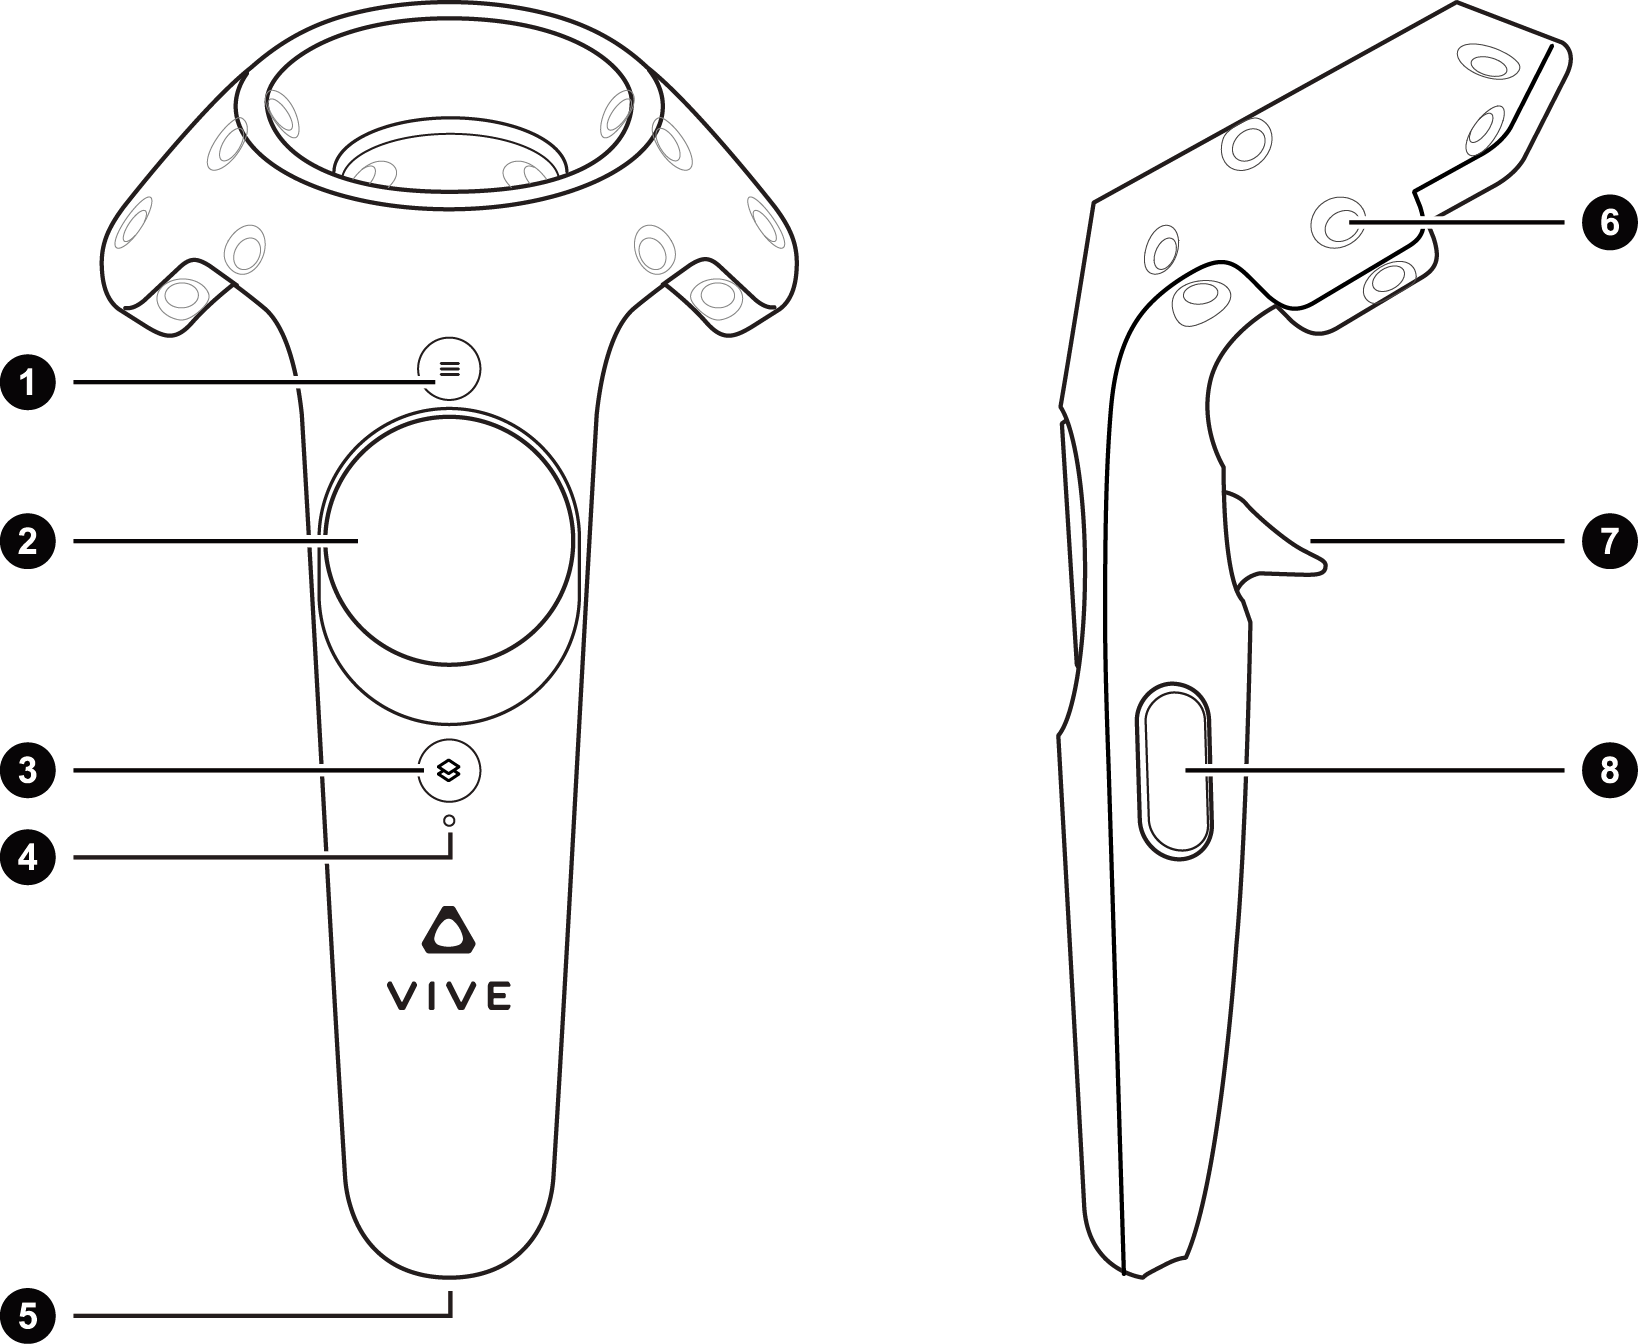
\includegraphics[width=\textwidth]{ViveControllers}
 \caption{HTC Vive controllers}
 \label{fig:vive_controllers}
 % Taken from https://docs.unity3d.com/Manual/OpenVRControllers.html but can't find a good reference for it
\end{figure}

% TODO: ??? need to  be replaced with the relevant VR button 

\subsection*{Changing tools}
To change the currently used tool, a tool menu has to be opened first. This can be done by pressing ???, which will toggle the menu between the open and closed state. Closing and opening the menu again will always reopen it directly in front of the user. The tools can then be selected by pointing at the icon representing the desired icon and pressing ??? with the controller that should become that tool.

\subsection*{Saving and loading previous projects}
Saving and loading previous projects can be done via an additional menu which can be opened and closed by pressing ???. Similarly to the tool menu, it will always be opened directly in front of the user.

\subsection*{Example}
The example below will lead you through the process of creating a basic room and saving your progress:
\begin{enumerate}
    \item Move to the place where you want to start building your room by either physically walking over to that location or using the teleport tool. To use the teleport open the tool menu by pressing ??? and select a teleport tool by pointing at it with the laser and pressing ??? on the controller. The controller on which the ??? was pressed will be the controller that the teleport tool is assigned to and it'll be the controller that will be used to teleport.
    \item Change the tool to wall tool and use it to build 4 walls of your room forming a rectangle. If you closed the menu, or walked far away from it you can close it and reopen it by pressing ???. To build a wall point at the place you want it to start from and press and hold ???. Then point to the location where you want the wall to end and release the presses button. If you started the wall in the wrong place point at the sky to cancel that wall segment. The line drawn on the ground shows where the wall is going to be places, so you can see if it starts and ends in the desired location.
    \item Select the floor build tool from the tool menu. Press ??? to select 4 points on the ground that match up with the corners of your room. If you misplaced one of the points you can press ??? to cancel the last point. When the 4 points are places press ??? to confirm and create a new floor segment. The lines drawn show you where the floor you are creating now is going to be placed.
    \item To paint the floor, change to tool o the paint floor tool and point at the floor you want to paint. Press ??? to toggle between the textures and ??? to apply the texture to the floor that is being pointed at. The same tool can be used to apply different textures to objects as well.
    \item To add objects to the scene select the add object tool. The green ghost object will show you where the object is going to be places. You can rotate it using ???, reset the rotation by pressing ???, change the object with ??? and confirm the placement with ???. The objects can be stacked on top of each other and can be automatically rotated to perpendicular position to the surface you're pointing at with ??? (for example making perpendicular to the wall rather than the floor).
    \item To add a doorway select the add doorway tool. To place a doorway point at the place in the wall where you want the doorway to be places and press ???. Once placed doorway cannot be removed and multiple doorways can be joined together to create a wider passage. To place a door use the add object tool.
    \item To add a ceiling change the floor level to one above the current one using ??? and create a floor with a floor build tool that corresponds to the area you want to be covered by the ceiling in the floor below. You can then use the floor painting tool to change the texture of the ceiling. You can then go back to the original floor by pressing ???; Alternatively if you are not planing on building future floor above, you can build a roof instead of a floor segment using the roof building tool.
    \item To save the current project bring up the save/load menu by pressing ??? and select the save option from it with either controller by pointing at it and pressing ???.
    \item Exit the program and bring up the save/load menu. Press the load icon corresponding to your project by pointing at it with a controller and pressing ???.
\end{enumerate}